

\begin{figure}[t!]
\begin{center}
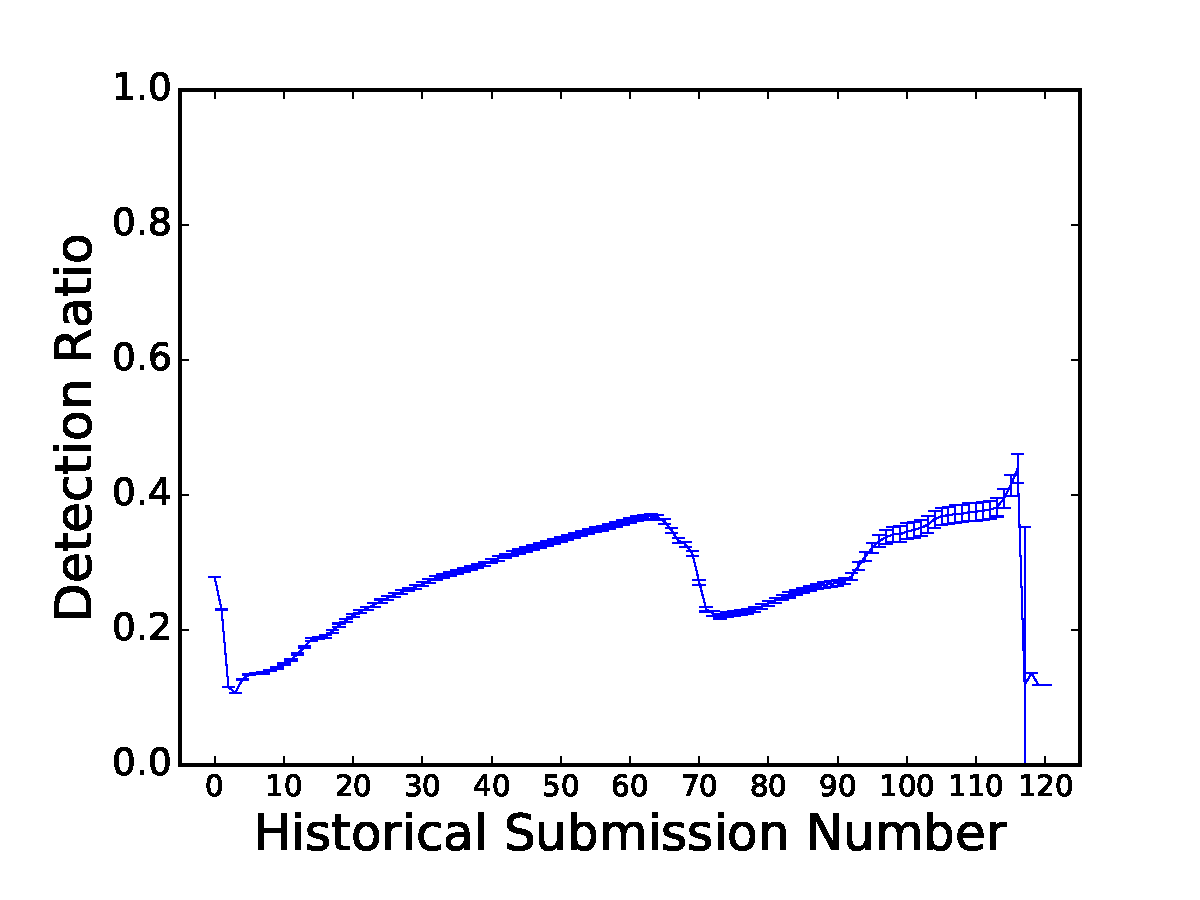
\includegraphics[width=2in]{figure/SubNum}
\caption{
The relation between historical submission number and detection rate.
(
How detection rate changes with historical submission number. 
Each historical submission number is rounded up to nearest 5.
95\% confidence interval is also drawn for each point.
)	
}
\label{fig:hisnum}
\end{center}
%\vspace{-0.25in}
\end{figure}

%\begin{figure}[t!]
%\begin{center}
%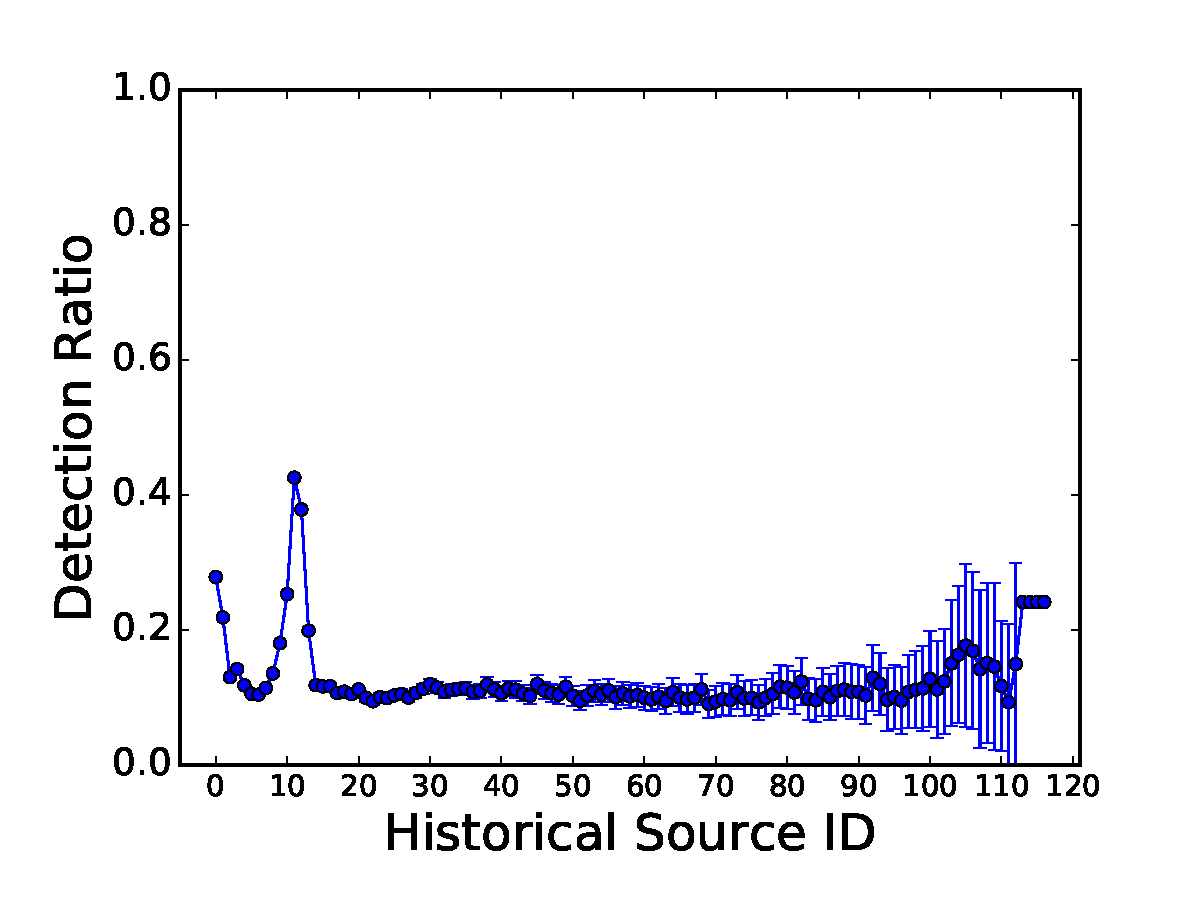
\includegraphics[width=2.5in]{figure/SubID}
%  \mycaption{fig:hisid}{The relation between the number of historical source ids and detection rate.}
%{\footnotesize{(How detection rate changes with the number of historical source ids. 
%Each historical number of source ids is rounded up to nearest 5.
%95\% confidence interval is also drawn for each point.)}}

%\end{center}
%\vspace{-0.25in}
%\end{figure}
